\documentclass[12pt,a4paper]{article}
\usepackage{../lecture-notes/vkCourseML}
\usepackage{url}
\title{Машинное обучение, ФКН ВШЭ\\Семинар №25\\Интерпретируемость моделей}
\begin{document}
\author{}
\date{}
\maketitle

\section{Введение}

Ранее в курсе мы рассматривали различные модели машинного обучения, основной задачей которых является сделать предсказание, <<хорошее>> с точки зрения некоторых функционалов качества. Чаще всего модели не могут сделать идеальных предсказаний (из-за шума в данных или отсутствия реальной функциональной зависимости между признаками и целевой переменной). В некоторых задачах ошибка не так критична (например, в ранжировании фильмов в рекомендациях) и может вызвать лишь небольшой негатив у пользователя. Однако есть задачи, в которых цена --- человеческие жизни или хотя бы большие суммы денег.

В случае, когда от модели зависит выбор способа лечения при диагностировании заболевания, становится важным понимать, почему модель приняла то или иное решение. По законам некоторых стран нельзя принимать решение о выдаче кредита на основании модели, объяснить которую невозможно.

Также иногда в процессе разработки модели может быть полезно лучше понимать, на какие данные она <<обращает внимание>>. Так можно найти ошибки в реализации подсчёта признаков (признаки не используются или используются не так, как ожидалось) или найти ошибки в данных (например, утечки целевой переменной).

На этом семинаре рассмотрим несколько подходов к интерпретации моделей.

\section{Интерпретация, основанная на особенностях моделей}

Некоторые модели из-за своих особенностей позволяют понять, какие признаки вносят наибольший вклад при построении предсказаний. Рассмотрим несколько из них.

\subsection{Линейные модели}
\par Естественной важностью признаков в линейных моделях являются веса признаков (после маштабирования). По абсолютному значению можно судить о силе влияния на предсказание, а по знаку "--- на направление. Однако в случае большого количества признаков или при наличии взаимосвязи между признаками могут быть искажения (например, два скоррелированных признака разделят между собой важность, а иногда один из них может иметь противоположный знак).

\subsection{Решающие деревья}
	\par Исключительной особенностью деревьев является простота их интерпретации (кроме того, их можно еще и визуализировать), однако при переходе к композициям над решающими деревьями (например, случайному лесу или бустингу) интерпретировать и визуализировать тысячи деревьев уже не представяется возможным.
	
\subsection{Нейронные сети}
	\par Для нейронных сетей, строящих предсказания для изображений, можно строить карты уверенности предсказаний. Для этого <<закрывается>> некоторый элемент исходного изображения и сравнивается уверенность предсказания по сравнению с исходным изображением "--- чем сильнее она уменьшилась, тем важнее для предсказания пиксели из <<закрытой>> части изображения, поэтому разность уверенностей можно использовать в качестве важностей различных элементов исходного изображения. На основании этих разностей можно строить тепловую карту важности пикселей для предсказания (пример на рис.~\ref{neuro_heatmap}). В качестве <<закрывания>> части изображения можно использовать её размытие или замену пикселей из этой части на однотонные.

	\begin{center}
	\begin{figure}[!htb]
	 \centering
	 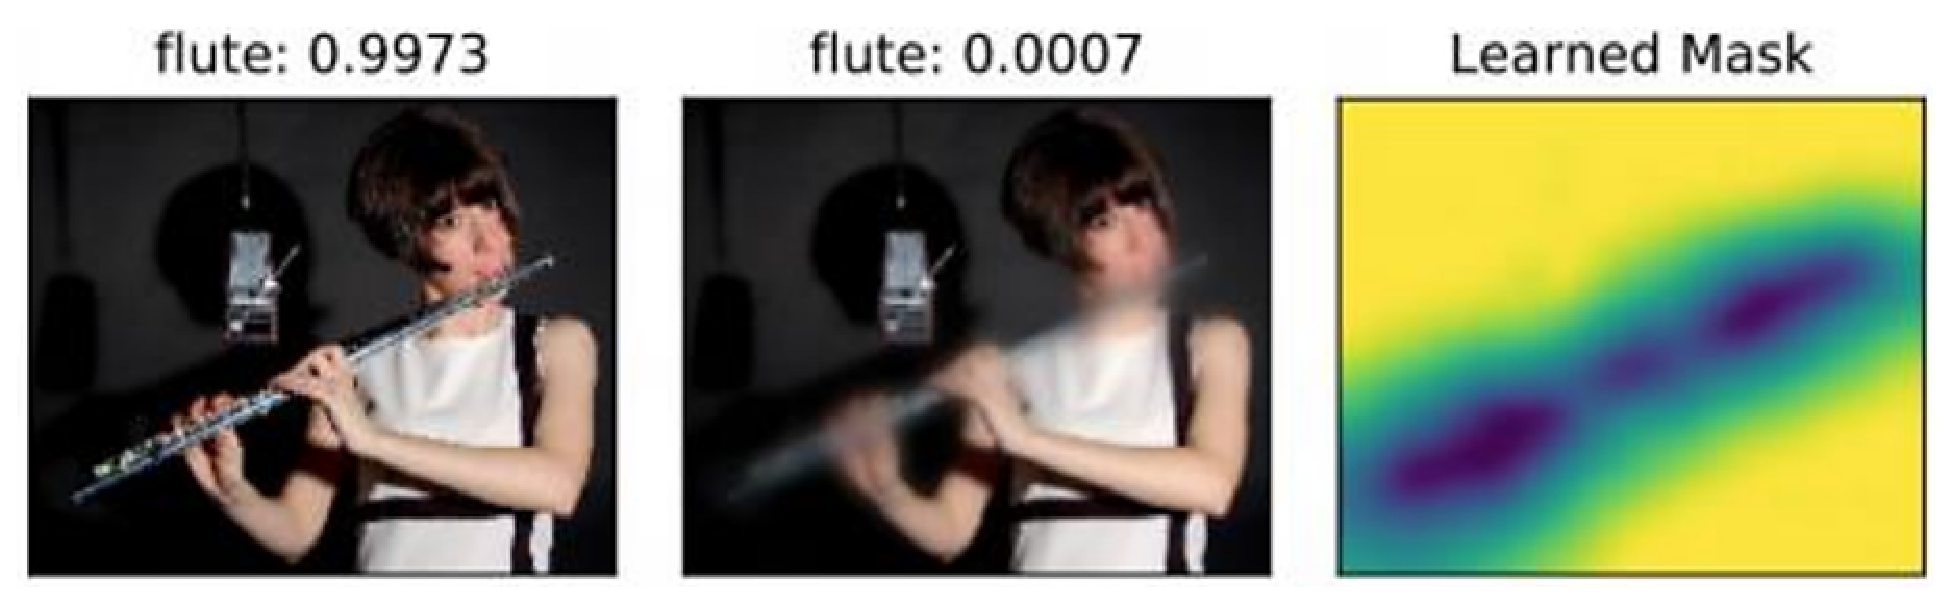
\includegraphics[width=1.0\linewidth]{neuro_heatmap.eps}
	 \caption{Пример построения тепловой карты на изображении для нейронной сети}
	 \label{neuro_heatmap}
	\end{figure}
	\end{center}

\section{LIME}

	\par Рассмотрим метод \textbf{LIME} (\emph{Local Interpretable Model-Agnostic Explanations}), основная идея которого, как следует из названия, заключается в том, чтобы интерпретировать предсказания некоторой \textbf{объясняемой} модели~$a(x)$ для заданного объекта~$x^*$ в его окрестности.
	\par Предполагается, что полученная интерпретация может использоваться широким кругом лиц для принятия решений (например, докторами для принятия решений о лечении пациентов), поэтому для каждого объекта наряду с признаковым описанием $x$, используемым в модели~$a(x)$, вводится его \emph{интерпретируемое} представление~$\bar{x}$, а результатом работы метода является \textbf{объясняющая} модель~$\bar{a}(\bar{x}),$ строящая предсказания именно для этих интерпретируемых представлений (а не для исходных признаковых описаний объекта). В связи с этим в качестве интерпретируемых представлений обычно рассматривают достаточно простые бинарные признаковые описания исходных объектов, например:
	\begin{itemize}
		\item для текстовых данных можно использовать <<мешок слов>> с ограничением на количество слов или $N$-грамм, используемых в представлении;
		\item для изображений используется аналогичное представление, но вместо слов выступают \emph{суперпиксели} — непрерывные области <<похожих>> пикселей, которые могут быть найдены на изображении~$x$ при помощи любого стандартного метода сегментации изображений.
	\end{itemize}

	\begin{center}
	\begin{figure}[!htb]
		\centering
		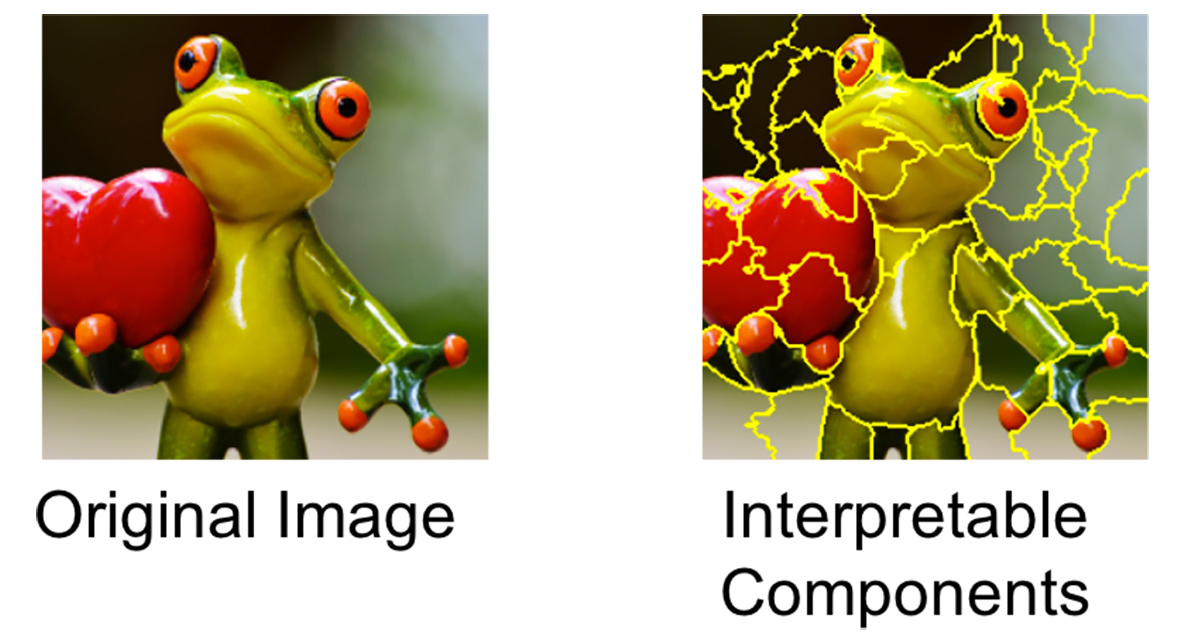
\includegraphics[width=0.8\linewidth]{superpixels.eps}
		\caption{Пример разбиения изображения на суперпиксели}
	\end{figure}
\end{center}


	\par Для построения объясняющей модели~$\bar{a}(\bar{x})$ составляется <<суррогатная>> выборка $X_{x^*}^\ell = \{ (\bar{x}_i, y_i) \}\}$ следующим образом: создадим объект~$\bar{x}_i$ путем случайного обнуления случайного количества единиц (все случайности — согласно равномерным распределениям) в интерпретируемом представлении~$\bar{x}^*$ объекта, для которого строится интерпретация, после чего перейдем от представления $\bar{x}_i$ нового объекта к признаковому описанию~$x_i$ в исходном признаковом пространстве и положим $y_i = a(x_i)$. Таким образом, мы создали искусственную выборку в окрестности интерпретируемого представления $\bar{x}^*$, после чего для каждого объекта вычислили таргет как прогноз интерпретируемой модели $a(x)$ в исходном признаковом пространстве (в случае многоклассовой классификации интерпретация чаще всего строится независимо для каждого класса).
	\par Обратим внимание на переход от интерпретируемого представления~$\bar{x}_i$ к исходному признаковому описанию~$x_i$: для текстов под <<обнулением>> элементов представления понимается удаление соответствующих слов или $N$-грамм из исходного текста и вычисление нового признакового описания для изменённого текста; для изображений аналогично подразумевается <<закрытие>> соответствующих суперпикселей изображения.
	
	\begin{center}
		\begin{figure}[!htb]
			\centering
			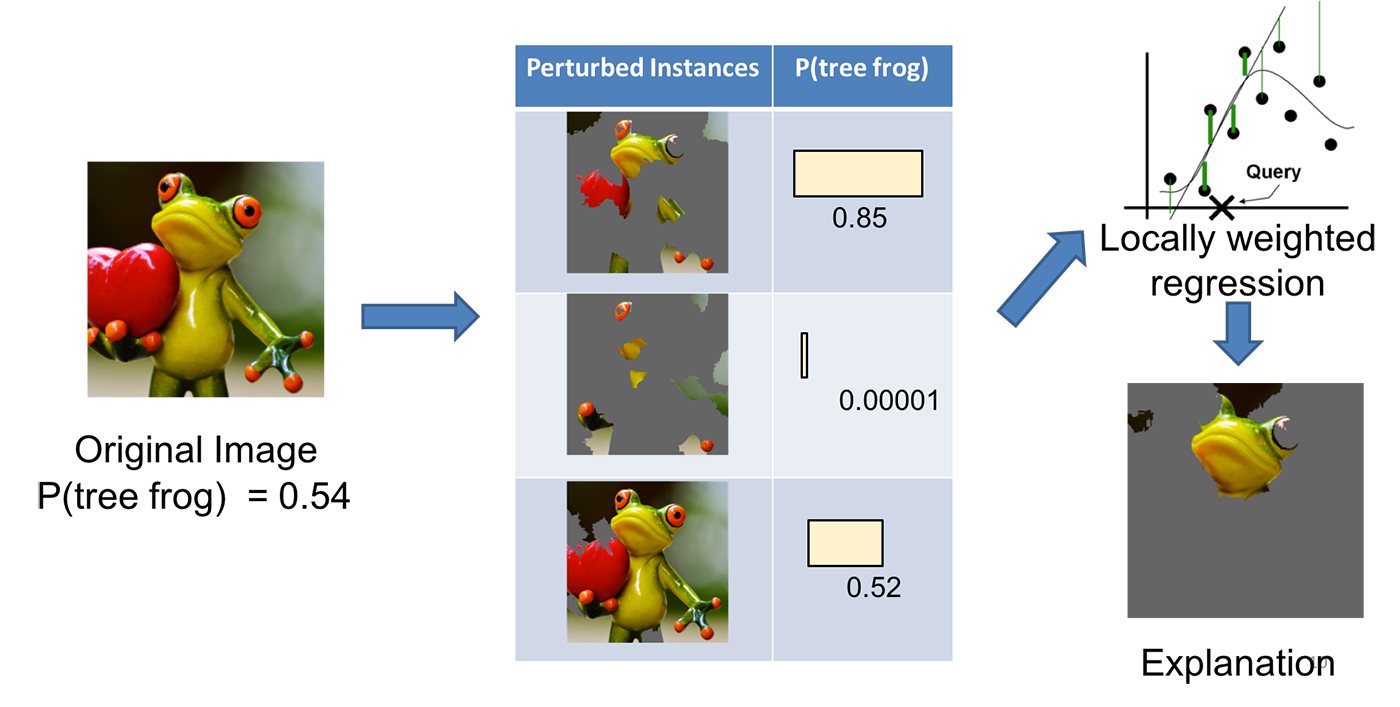
\includegraphics[width=0.9\linewidth]{lime_sample.eps}
			\caption{Пример генерации объектов для суррогатной выборки: из исходного изображения случайным образом удаляется часть суперпикселей, для полученного изображения вычисляется прогноз модели, после чего на итоговой взвешенной выборке интерпретируемых бинарных представлений обучается объясняющая модель}
		\end{figure}
	\end{center}
	
	\par Поскольку итоговая модель $\bar{a}(\bar{x})$ должна, во-первых, интерпретировать предсказания в окрестности исходного объекта, и, во-вторых, быть достаточно простой, то она может быть найдена как решение, например, следующей задачи:
	\[
	\bar{a} = \argmin_{b \in B} \sum_{\bar{x}_i \in X_{x^*}^\ell} \pi_{x^*} (x_i) (a(x_i) - b(\bar{x}_i))^2 + \Omega(b),
	\]
	
	где $x^*$ — объект, для которого происходит поиск интерпретации, 
	\par $B$ — семейство возможных объясняющих моделей (ещё раз обратим внимание на то, что эти модели строят предсказания для интерпретируемых представлений, а не для исходных признаковых описаний), 
	\par $\pi_{x^*}(x_i)$ — вес объекта в функционале ошибки (часто в качестве $\pi_{x^*}(x)$ выбирают некоторое ядро в центром в объекте $x^*$), 
	\par $\Omega(b)$ — сложность объясняющей модели. 
	\par В качестве семейства объясняющих моделей~$B$ можно выбирать любое семейство достаточно простых моделей (например, линейные модели, решающие деревья или решающие списки), в качестве функции потерь можно также выбирать любую другую вместо квадратичной, используемой в формуле выше. Частный случай LIME при использовании квадратичной функции потерь с экспоненциальным ядром в качестве функции $\pi_{x^*}(x)$, а также семейства $B$ линейных моделей и $\Omega(b) = \infty [\| w_b\|_0 > K],$ где $w_b$ "--- вектор весов для модели~$b$ (то есть с ограничением количества ненулевых весов модели), называется методом \emph{разреженных линейных представлений} (\emph{Sparse Linear Explanations}) и на практике используется чаще всего.
	\par После нахождения объясняющей модели~$\bar{a}(\bar{x})$ в силу того, что она строит прогнозы для бинарных векторов, а также того, что является достаточно простой в силу выбора семейства и наличия регуляризации $\Omega(b)$, она может быть легко интерпретирована — например, в случае метода Sparse Linear Explanations в качестве интерпретации достаточно предъявить список признаков с ненулевыми весами (в случае текстов и изображений эти признаки говорят о наличии слов/$N$-грамм и суперпикселей соответственно).

%Построение суррогатной модели происходит по следующей схеме:
%
%\begin{enumerate}
%	\item Выбрать объект $x$, в окрестности которого производится аппроксимация.
%	\item Сгенерировать новые объекты в окрестности объекта $x$.
%	\item Обучить объясняющую модель на сгенерированных точках (с учётом ограничения на сложность).
%	\item Интерпретировать обученную объясняющую модель.
%\end{enumerate}
%
%Способ получения новых сгенерированных объектов зависит от их типа:
%
%\begin{enumerate}
%	\item Для текстовых данных в случае Bag-of-words представления можно исключать отдельные слова из объекта $x$ (аналогично бинарные данные).
%	\item Для изображений можно отключать часть пикселей из объекта $x$.
%	\item Для табличных данных с вещественными признаки генерируются новые объекты, в которых признаки искажаются в соответствии с нормальным распределением вокруг объекта.
%\end{enumerate}

\begin{center}
\begin{figure}[!htb]
 \centering
 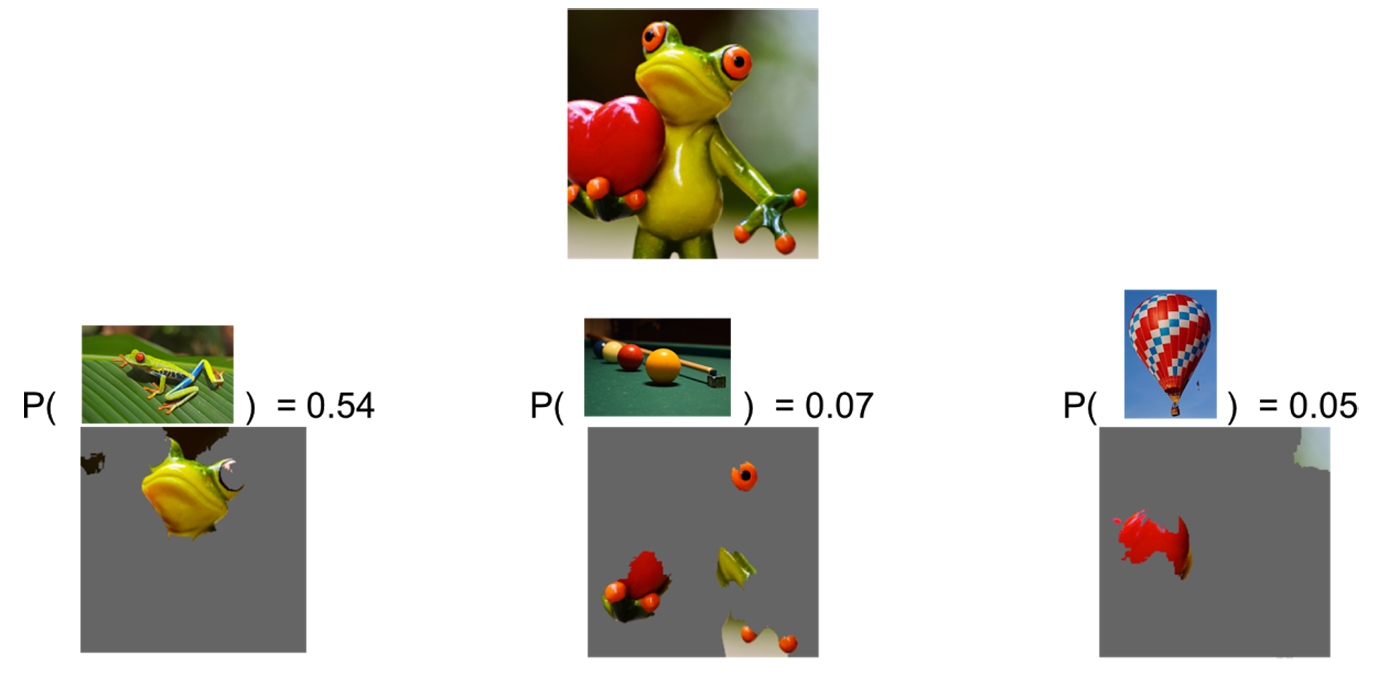
\includegraphics[width=0.9\linewidth]{lime_result.eps}
 \caption{Пример работы LIME для описания 3 классов}
\end{figure}
\end{center}

%Каждому сгенерированному объекту могут приписываться веса, с которыми они входят в функцию потерь $L$. Эти веса обычно рассчитываются с помощью ядер как расстояние от сгенерированного объекта до объекта $x$.
%
%У LIME существуют проблемы с данными большой размерности или с признаками коррелирующими друг с другом. Для табличных данных предполагается отсутствие взаимосвязей между признаками, что далеко не всегда верно.


\section{Influential Instances (влиятельность объектов)}

Альтернативой подходу с оценкой влияния признаков и их изменения на предсказания объясняемой модели является подход с оценкой влияния объектов обучающей выборки на построенную модель. Существует два подхода для оценки влияния объектов: через удаление объекта из обучающей выборки и через оценку влияния на функцию потерь.

Оценка влияния объектов на модель помогает ответить на вопросы об устойчивости моделей (хорошая модель не должна сильно зависеть от отдельных объектов) и найти особенности в данных, которые могут мешать настройке модели (модели, плохо устойчивые к выбросам, сильно изменяются при их удалении).

\subsection{Диагностика через удаление}

Для оценки влиятельности объекта обучим модель 2 раза: на полной обучающей выборке и на обучающей выборке без этого объекта, после чего оценим, насколько полученные модели отличаются друг от друга. Если у модели есть явный вектор параметров, то можно посчитать отличия в векторах параметров (например, как норму разности). Более универсальный подход заключается в сравнении предсказаний двух моделей, например, с помощью \emph{расстояния Кука} (\emph{Cook's distance}). Для задачи регрессии влияние объекта~$x_i$ обучающей выборки~$X^\ell$ можно оценить следующим образом:

$$
D_i = \frac{\sum_{j=1}^\ell (a(x_j) - a^{-i}(x_j))^2}{d \times \text{MSE}(a, X^\ell)},
$$

где $a(x)$ "--- модель, обученная на полной обучающей выборке $X^\ell$, $a^{-i}(x)$ "--- модель, обученная на выборке $X^\ell \, \backslash \, \{(x_i, y_i)\}$,  $d$ --- количество признаков, $\text{MSE}(a, X^\ell)$ --- исходная квадратичная ошибка модели $a(x)$ на выборке $X^\ell$.

На практике поиск влиятельных объектов может быть малоинформативным, поскольку сложно интерпретировать таблицу с признаками десяти самых влиятельных объектов. Однако можно построить простую модель (например, решающее дерево), которая будет детектировать эти влиятельные объекты относительно всех остальных объектов. Так можно будет увидеть, чем эти влиятельные объекты отличаются от остальной выборки.

Также можно оценивать влиятельность конкретного объекта на предсказание для другого объекта, оценивая разность от предсказаний двух моделей.

\subsection{Функции влияния (influence functions)}

Недостатком подхода с удалением является его сложность "--- на практике обучить модели по количеству объектов в обучающей выборке не представляется возможным. Альтернативный вариант предлагает для моделей с дифференцируемой функцией потерь исследовать влияние изменения веса для конкретного примера обучающей выборки на параметры модели через влияние на функцию потерь.

Обозначим за $\hat{\theta}$ вектор параметров модели, обученной на выборке~$X^\ell$, \\за $\hat{\theta}_{\varepsilon, x_i}$~"---~вектор параметров модели при увеличении веса объекта $x_i$ на $\varepsilon$:

$$
\hat{\theta}_{\varepsilon, x_i} = \argmin_{\theta} \frac{1}{\ell} \sum_{i=1}^{\ell} L(x_i, \theta) + \varepsilon L(x_i, \theta)
$$

Заметим, что $\hat{\theta}_{0, x_i} = \hat{\theta}$. Тогда влияние увеличения веса объекта $x_i$ на ошибку на новом объекте $x$ можно вычислить следующим образом:

\begin{align}
I_{\text{up}, \text{loss}} (x_i, x)
& = \frac{ \partial L(x, \hat{\theta}_{\varepsilon, x_i})}{\partial \varepsilon} \Bigg|_{\varepsilon = 0}
= \nabla_\theta L(x, \hat{\theta}_{0,x_i})^\top \, \frac{d \hat{\theta}_{\varepsilon, x_i}}{d \varepsilon} \Bigg|_{\varepsilon = 0} \notag =\\
& = - \nabla_\theta L(x, \hat{\theta})^\top H_{\hat{\theta}}^{-1} \nabla_\theta L(x_i, \hat{\theta}), \tag{1} \label{up_loss}
\end{align}

где $H_{\hat{\theta}} = \frac{1}{\ell} \sum_1^\ell \nabla_\theta^2 L(x_i, \hat{\theta})$ "--- гессиан функции потерь $L$, который может быть вычислен приближённо. Кроме того, в последнем переходе мы воспользовались классическим результатом теории функций влияния о влиянии веса объекта на параметры модели, полное доказательство которого можно найти в~\cite{cook1982residuals}:
\[
	\frac{d \hat{\theta}_{\varepsilon, x_i}}{d \varepsilon}\Bigg|_{\varepsilon = 0} = - H_{\hat{\theta}}^{-1} \nabla_\theta L(x_i, \hat{\theta}).
\]
Интуиция за этой формулой~\ref{up_loss} следующая. Представим гессиан равным единичной матрице, тогда положительное значение $I_{\text{up}, \text{loss}} (x_i, x)$ (т.е. ухудшение качества предсказания на объекте~$x$) означает противоположные направления градиентов функции потерь для объектов $x_i$ и $x$ (то есть объект $x_i$ <<мешает>> построению хорошего прогноза на $x$).

%\begin{center}
%\begin{figure}[!htb]
% \centering
% \includegraphics[width=0.9\linewidth]{influence-functions-svm-inception.jpg}
% \caption{Визуализация поиска влиятельных изображений для задачи классификации картинок на рыбы и собаки. Для метода опорных векторов влиятельные изображения это рыбы похожих цветов, а нейронная сеть обращает больше внимания на форму. Видно, что нейронная сеть ищет более сложные паттерны (большее евклидово расстояние между изображениями)}\label{fig:graph}
%\end{figure}
%\end{center}

Использовать функции влияния можно несколькими способами:
\begin{enumerate}
	\item Сравнивать модели между собой. Как в примере с изображением, может получиться так, что одна из моделей ищет более сложные паттерны на изображении по сравнению с другой. Для этого нужно сравнивать между собой наиболее влиятельные изображения для некоторого примера выборки.
	\item Детектирование несовпадений доменов между обучающим и тестовым множеством. Можно найти ложное срабатывание модели и изучить влиятельные объекты для этого ложного предсказания. Так можно выяснить паттерны в данных, которые мешают корректной работе алгоритма на новом домене данных (данные из несколько другого распределения).
	\item Коррекция обучающих данных. Если у нас есть возможность перепроверить корректность разметки небольшого числа объектов обучающей выборки, то эффективнее сделать это на наиболее влиятельных объектах, так как именно они влияют на нашу модель сильнее всего.
\end{enumerate}


\section{Состязательные атаки}

Кроме интерпретации модели для оценки её устойчивости через признаки или объекты обучающей выборки, можно оценивать корректность модели через её устойчивость к состязательным (\emph{adversarial}) объектам. Состязательными объектами называют такие объекты, предсказания на которых радикально меняются при малом изменении исходных данных (например, после наложения шума на корректно классифицируемое изображение панды нейросеть может уверенно относить новое изображение к совершенно другому классу).

\begin{center}
	\begin{figure}[!htb]
		\centering
		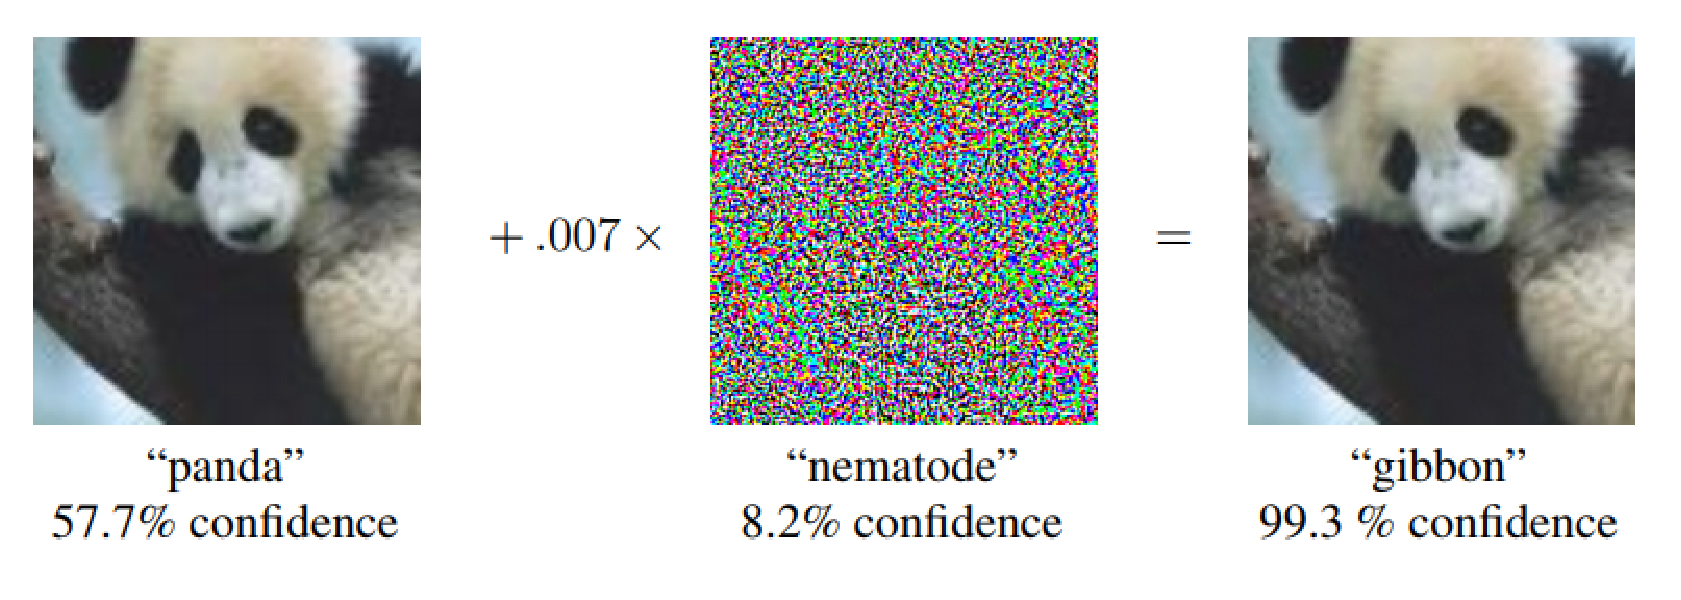
\includegraphics[width=0.9\linewidth]{adversarial_attack.eps}
		\caption{Пример состязательного изображения}
	\end{figure}
\end{center}


\par Методы генерации таких изображений называются состязательными атаками (\emph{adversarial attacks}). Целью атак является изменение заданного объекта таким образом, чтобы изменение было не слишком <<заметным>> и чтобы при этом изменить предсказание заданной модели для него. Чтобы контролировать <<заметность>> изменения, исходное и измененное изображение обычно сравнивают по некоторой метрике (чаще всего в качестве метрики выбирают $l_{\infty}$, то есть учитывается максимальное по всем пикселям изменение исходного изображения).
\par В основном все методы делятся на две группы: \emph{white-box} (с доступом к градиенту модели) и \emph{black-box} (как мог догадаться смышлёный читатель, без доступа к градиенту модели). Кроме того, атаки делятся на ненаправленные (\emph{non-targeted}), целью которых является заставить модель строить \emph{какой угодно} некорректный прогноз для измененного объекта (например, отнести изображение кошки к любому классу, отличному от кошек), и направленные (\emph{targeted}), целью которых является заставить модель строить некий \emph{определенный} некорректный прогноз (например, отнести изображение к конкретному классу <<собака>>).
\newpage
\par В рамках атаки, можно, например, можно генерировать объект, решая следующую оптимизационную задачу:

$$
L(a(x^{adv}), y_{\text{target}}) + \lambda \lVert x^{adv} - x \rVert \to \min_{x^{adv}},
$$

где $x$ "--- атакуемое изображение, $x^{adv}$ "--- состязательный объект, который мы хотим построить на основе $x$, $L$ "--- функция потерь нашей модели, $a(x)$ "--- модель, $y_{\text{target}}$ "--- желаемая метка объекта $x^{adv}$.

\par Пусть $x$ "--- исходное изображение, для которого производится атака, $y_{\text{true}}$ "--- его истинная метка. Разберем несколько широко используемых состязательных white-box атак.
\begin{enumerate}
	\item \textbf{Fast gradient sign method} (FGSM)\\
	Ненаправленный метод атак, идея которого заключается в том, чтобы изменить объект в сторону градиента функции потерь~$L$ для истинной метки объекта:
	\[
		x^{adv} = x + \varepsilon \sign (\nabla_x L(x, y_{\text{true}})).
	\]
	Заметим, что при таком способе изменения исходного изображения $l_\infty$-норма их разности не будет превышать~$\varepsilon,$ поэтому мощность атаки может регулироваться этим гиперпараметром. Данный метод является ненаправленным, а также относится к т.н. одношаговым (\emph{one-shot}) методам.
	\item \textbf{Targeted fast gradient sign method} (T-FGSM)\\
	Направленная версия \textit{FGSM}, в которой объект изменяется в сторону антиградиента функции потерь для целевой метки атаки $y_{\text{target}}:$
	\[
		x^{adv} = x - \varepsilon \sign (\nabla_x L(x, y_{\text{target}})).
	\]
	\item \textbf{Iterative fast gradient sign method} (I-FGSM)\\
	В отличие от предыдущих методов, являющихся одношаговыми, в данном вместо одного шага длины $\varepsilon$ делается $T$ шагов длины $\alpha = \frac{\varepsilon}{T}:$
	\begin{align}
		&x_0^{adv} = x \notag,\\
		&x_{t+1}^{adv} = x_t^{adv} + \alpha \sign (\nabla_x L(x, y_{\text{true}})) \notag
	\end{align}
\end{enumerate}


В случае с black-box атаками необходимо обучить суррогатную модель на выборке, таргетами в которой являются предсказания атакуемой модели (<<чёрного ящика>>), после чего для полученной модели проводится атака white-box методами.

\nocite{ribeiro2016should}
\nocite{medium_adversarial}
\bibliographystyle{unsrt}
\bibliography{sem25-interpreting}
\end{document}
